\chapter{Synthese mit reinen Tönen}


\begin{enumerate}[a)]
% a)
\item Siehe MATLAB-Code:
\begin{itemize}
\item
SineSynth.m
\end{itemize}
\item
Siehe MATLAB-Code:
\begin{itemize}
\item
SineSynth.m
\end{itemize}
\vspace{\baselineskip}
Um die zeitliche Hüllkurve zu realisieren, verwenden wir ein in zwei Hälften geteiltes Hann-Window, welches als Attack und Decay für einen reinen Sinuston fungiert. Der ansteigende Teil entspricht der Formel
\begin{align*}
w(n) &= 0.5 \cdot (1- \mathrm{cos}(2 \pi \frac{n}{N})) \\
n &= 0\,...\,N/2
\end{align*}
und der abklingende Teil derselben Formel in einem anderen Wertebereich:
\begin{align*}
w(n) &= 0.5 \cdot (1- \mathrm{cos}(2 \pi \frac{n}{N})) \\
n &= N/2+1\,...\,N
\end{align*}
\begin{figure}
  \centering
      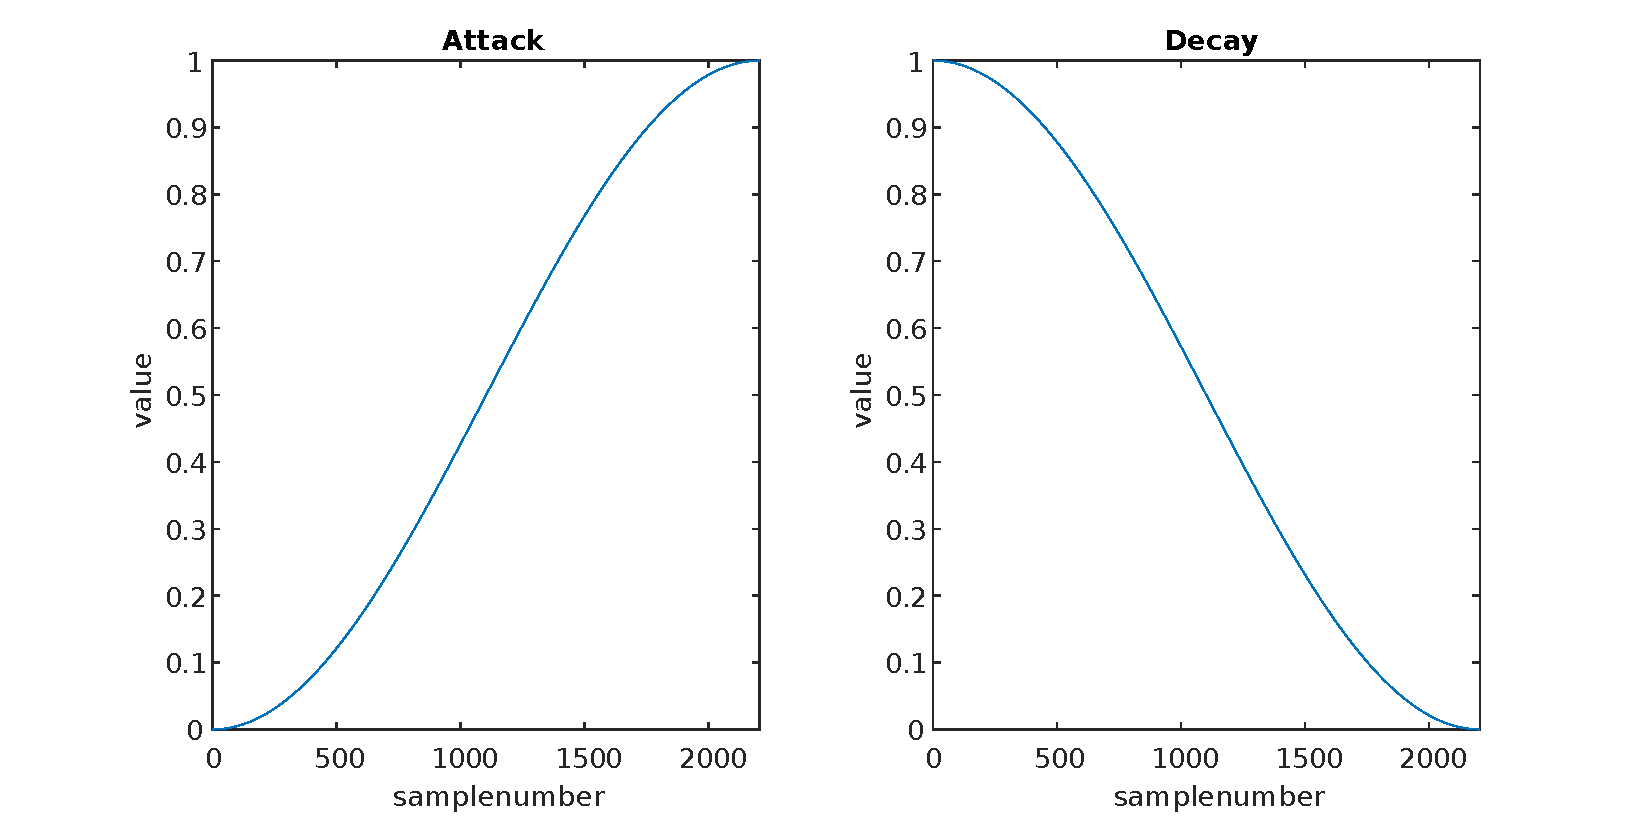
\includegraphics[width=\textwidth]{Figures/envelopeplot}
 \caption{In zwei Hälften geteiltes Hann-Fenster für die zeitlichen Attack- und Decay-Hüllkurven der Sinustöne. Länge: t = 0.05 s bei fs = 44100 Hz}
	\label{fig:env}
\end{figure}
\end{enumerate}
